\section{Introduction}
Developing quality code is essential 
Code quality can be subjective, each person and organisation will have differing needs and wants when it comes to the quality of their code. But there are a many well defined areas that are as universal as can be.

The current progress is mostly research and planning with some small time taken to make prototypes although these have not gotten far.
\newline
\begin{figure}
  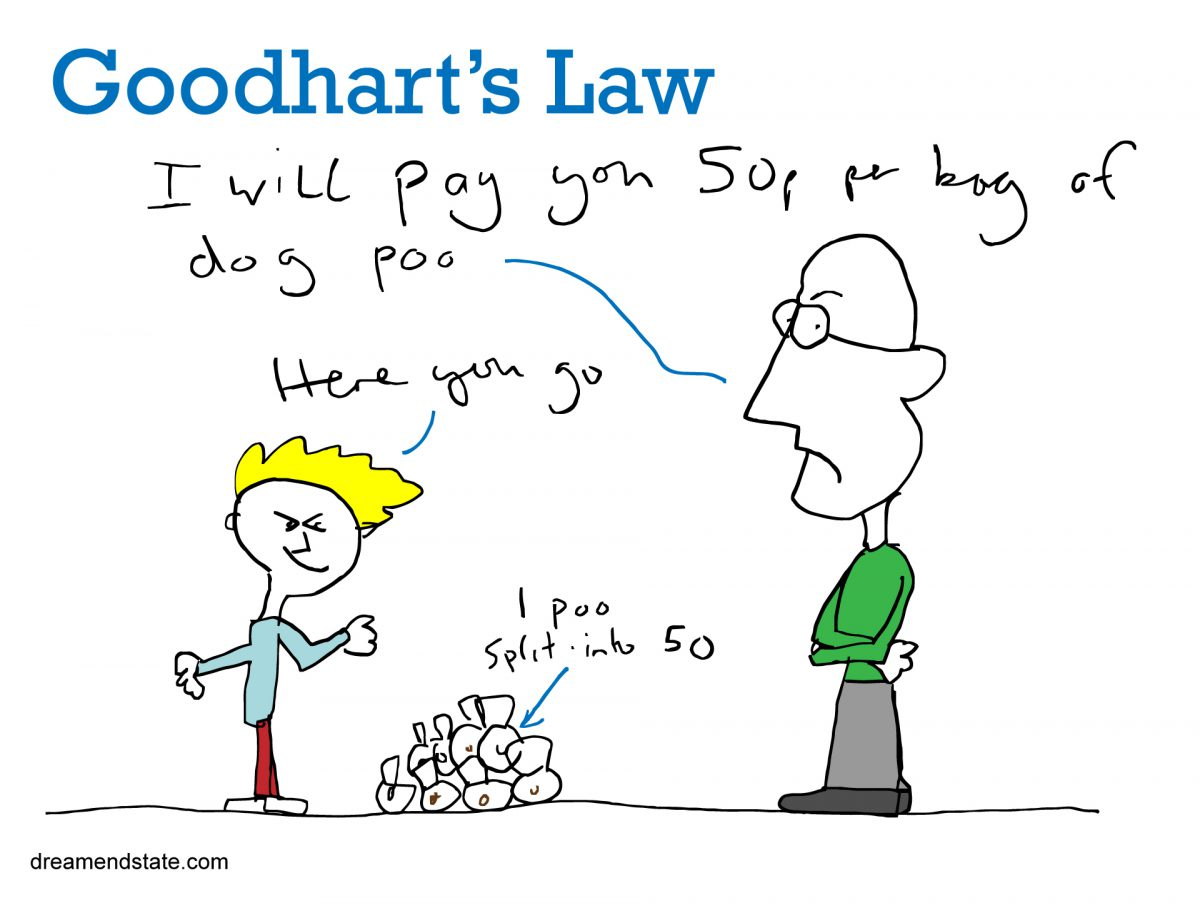
\includegraphics[width=.2\textwidth]{images/goodhart-1200x903.jpg}
  \caption{Goodharts law}
  \Description{Setps of code analyser}
  \label{fig:goodhart}
\end{figure}
One stumbling block was the realisation that quantitising the quality of code can be a trap, illustrated by the figure above.
\begin{verbatim}
  Goodhart's Law 
  "When a measure becomes a target, 
  it ceases to be a good measure"
\end{verbatim}
This has been the main part of my research, ensuring the measures I use are difficult to be gamed rather than completed.
\newline
The main stumbling block occured were understanding the depth of which static analysis needs to be, to ensure it is correct, this involves following similar steps to a compiler without producing a program.

\begin{figure}
  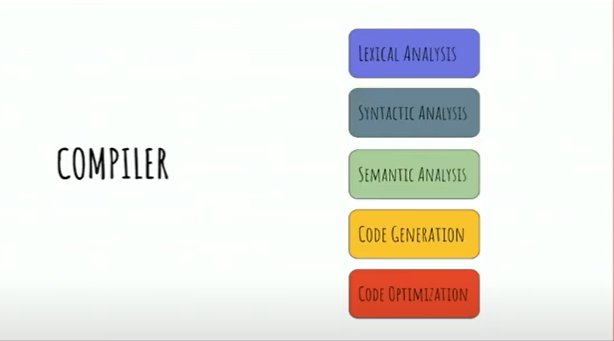
\includegraphics[width=.2\textwidth]{images/compiler.png}
  \caption{Compiler}
  \Description{Setps of compiler}
  \label{fig:comp}
\end{figure}
\begin{figure}
  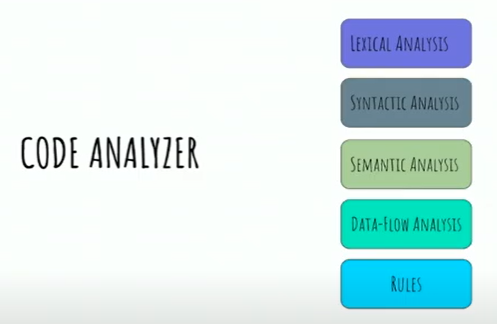
\includegraphics[width=.2\textwidth]{images/code-analyser.png}
  \caption{Code analyser}
  \Description{Setps of code analyser}
  \label{fig:codeanalyser}
\end{figure}

In the figures above you can see that the early steps of a code analyser and a compiler are very similar. Performing these steps completely means that we can be sure that the source code is being parsed correctly and and proceed with analysis on our tokenised tree.



